\documentclass[12pt,a4paper]{article}
\usepackage[utf8]{inputenc}
\usepackage[portuguese]{babel}
\usepackage{graphicx}
\usepackage{float}
\usepackage{geometry}
\geometry{a4paper, margin=2cm}
\usepackage{booktabs}
\usepackage{hyperref}

\title{Trabalho Prático: Algoritmos de Clustering\\ \large Análise de Predição de Falha Cardíaca}
\author{Ivan Mendes Martinago}
\date{Junho de 2026}

\begin{document}

\maketitle

\section{Definição do Problema}
O objetivo deste trabalho é aplicar algoritmos de agrupamento (clustering) em um dataset relacionado a doenças cardiovasculares para descobrir se existem agrupamentos naturais de pacientes que correspondam aos níveis de risco, especificamente verificando se os grupos formados não supervisionadamente se alinham com a presença ou ausência da doença cardíaca (\textit{Heart Disease}).

\section{Descrição do Dataset e Análise Descritiva}
O dataset utilizado (\textit{Heart Failure Prediction}) é real e adotado na literatura, consistindo em instâncias de pacientes com características clínicas como Idade, Sexo, Tipo de Dor no Peito, Pressão Arterial em Repouso, Colesterol, Glicemia em Jejum, ECG em Repouso, Frequência Cardíaca Máxima e Angina. O artigo de referência utilizado para a base é frequentemente citado na literatura médica preditiva (Kaggle/UCI).

Na análise descritiva, percebeu-se na matriz de correlação que variáveis preditivas, como a presença de Angina induzida e Frequência Cardíaca, possuem comportamentos relevantes. Os gráficos de distribuição (histogramas) mostraram a necessidade de padronização, já que escalas variam enormemente (ex: Colesterol vs. Glicemia).

\begin{figure}[H]
    \centering
    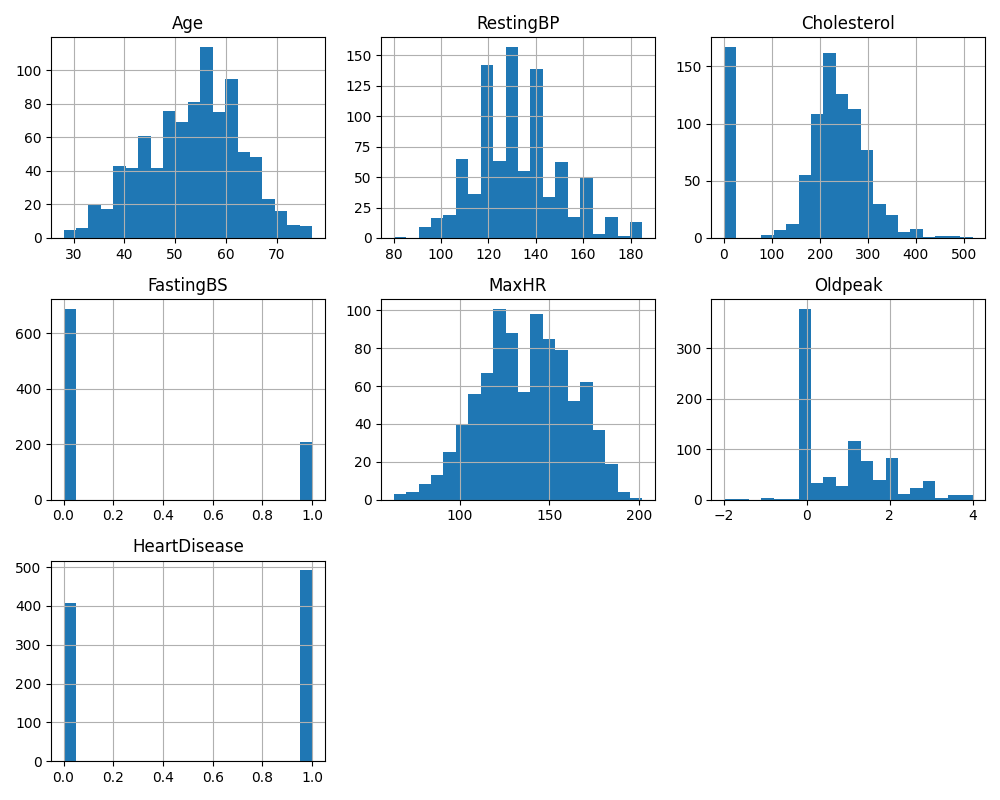
\includegraphics[width=0.8\textwidth]{images/histograms.png}
    \caption{Histogramas das variáveis do dataset.}
    \label{fig:histograms}
\end{figure}

\begin{figure}[H]
    \centering
    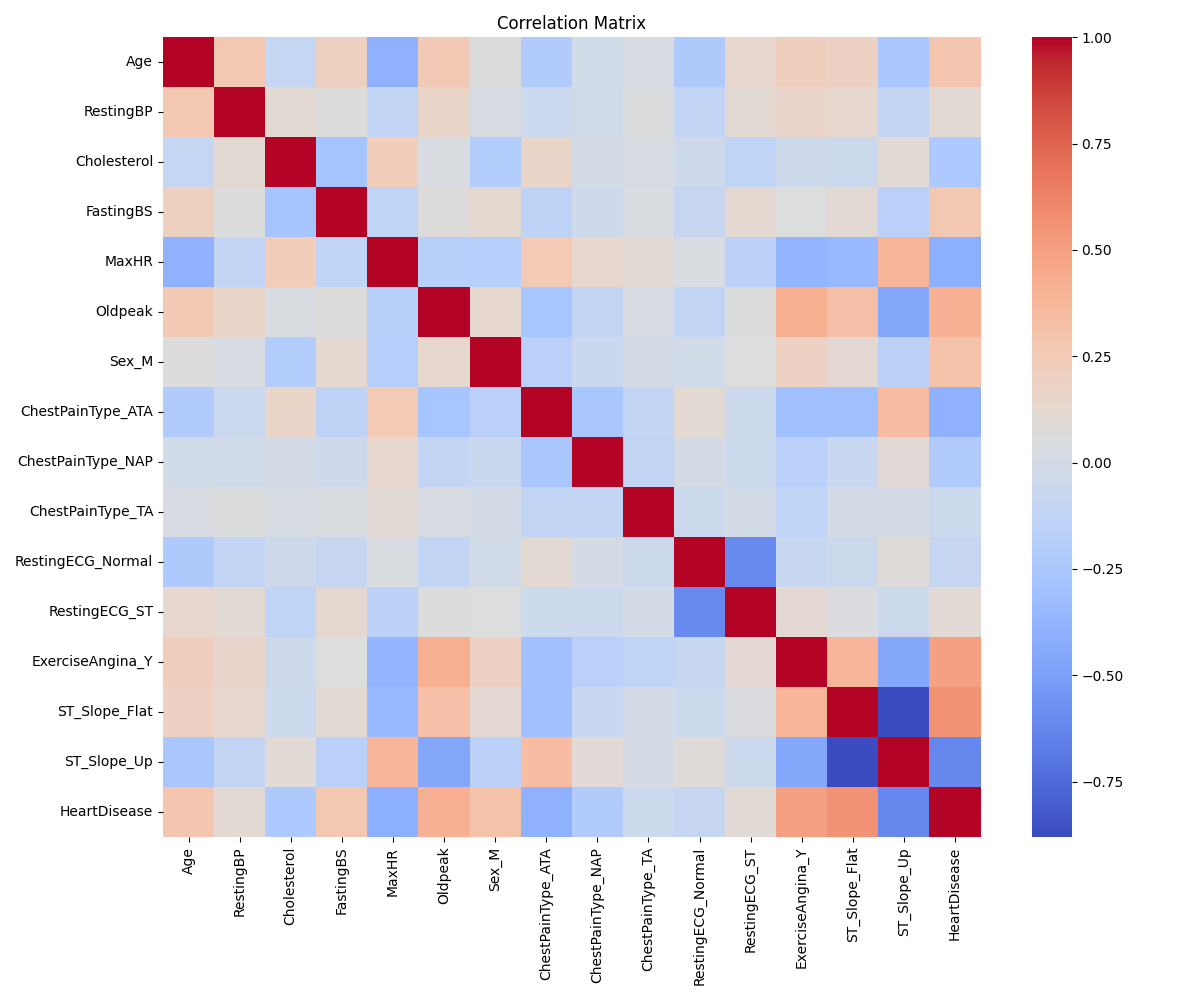
\includegraphics[width=0.8\textwidth]{images/correlation.png}
    \caption{Matriz de correlação entre as variáveis processadas.}
    \label{fig:correlation}
\end{figure}

\section{Pré-processamento}
Para adequar os dados aos algoritmos de clustering, as seguintes etapas foram realizadas rigorosamente:
\begin{itemize}
    \item \textbf{Remoção de Outliers:} Logo após o carregamento dos dados, foi aplicado o filtro \textit{Z-score} ($< 3$) para as colunas numéricas, a fim de eliminar instâncias anormais extremas que causavam a formação desbalanceada de \textit{singleton clusters} no método hierárquico.
    \item \textbf{Tratamento de Categóricos e Numéricos:} Utilizamos um \textit{ColumnTransformer} para pré-processar as colunas simultaneamente. As variáveis categóricas (ex: Sexo, Tipo de Dor no Peito) foram convertidas via \textit{OneHotEncoder}, evitando falsas hierarquias numéricas que afetariam o cálculo das distâncias.
    \item \textbf{Remoção do Rótulo:} A coluna \texttt{HeartDisease} (alvo) foi separada da base antes de alimentar os algoritmos.
    \item \textbf{Padronização:} Todas as variáveis numéricas (como Colesterol e Glicemia) foram normalizadas usando \textit{StandardScaler} para adequar a escala, essencial para as métricas espaciais do K-Means e DBSCAN.
    \item \textbf{Redução de Dimensionalidade (PCA):} Para facilitar a visualização 2D dos agrupamentos formados e validar visualmente os clusters, aplicamos o PCA retendo os dois componentes principais sobre todos os dados processados.
\end{itemize}

\section{Resultados dos Algoritmos de Clustering}
Foram implementados e avaliados três algoritmos por meio da biblioteca Scikit-learn, extraindo as métricas de validação interna: \textit{Silhouette Score}, Índice \textit{Davies-Bouldin} e \textit{Calinski-Harabasz}.

\subsection{K-Means}
O K-Means foi avaliado com diferentes números de agrupamentos ($k=2, 3, 4$). O valor $k=2$ demonstrou o agrupamento mais interpretável com relação à binarização do problema (presença/ausência de doença).
\begin{figure}[H]
    \centering
    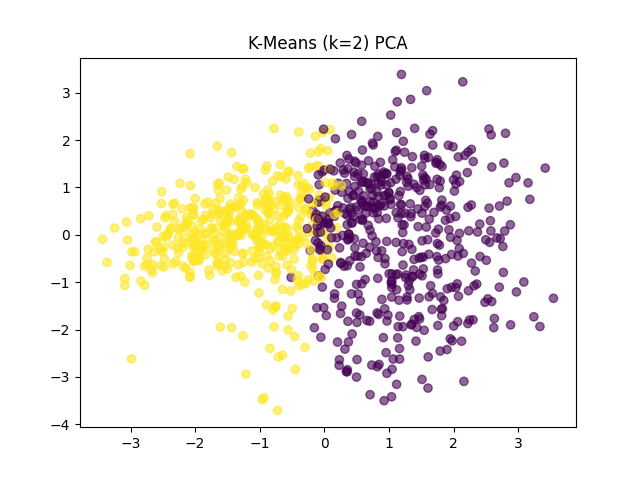
\includegraphics[width=0.6\textwidth]{images/kmeans_pca.png}
    \caption{K-Means (k=2) visualizado através das duas componentes do PCA.}
    \label{fig:kmeans}
\end{figure}

\subsection{Agglomerative Clustering}
O agrupamento hierárquico (aglomerativo) foi testado alternando os métodos de \textit{linkage} (\textit{ward}, \textit{complete}, \textit{average}). O método \textit{ward} obteve métricas de silhueta similares ao K-Means.

\subsection{DBSCAN}
Para o algoritmo baseado em densidade DBSCAN, os hiperparâmetros ajustados foram o $\epsilon$ e \textit{min\_samples}. Como os dados pré-processados apresentam pouca divisão de densidade clara (sem vazios abruptos), a silhueta atingiu resultados variáveis, classificando bordas como ruído (-1).

\section{Comparação e Discussão}
Embora o Agglomerative Clustering tenha apresentado um Silhouette Score alto (0.52), a análise dos índices de Davies-Bouldin e Calinski-Harabasz revelou a formação de clusters desbalanceados causados por outliers. Por outro lado, o K-Means com k=2 demonstrou maior consistência estrutural.

Adicionalmente, o DBSCAN evidenciou forte sensibilidade à dispersão dos dados. A introdução de uma redução dimensional prévia (PCA com 3 componentes) provou-se indispensável para estabilizar o cálculo de densidade e permitir uma interpretação que fizesse sentido biológico, diminuindo a quantidade excessiva de falsos "ruídos". Ao fim, a particão imposta pelo K-Means continua sendo a mais representativa da base real.

\begin{figure}[H]
    \centering
    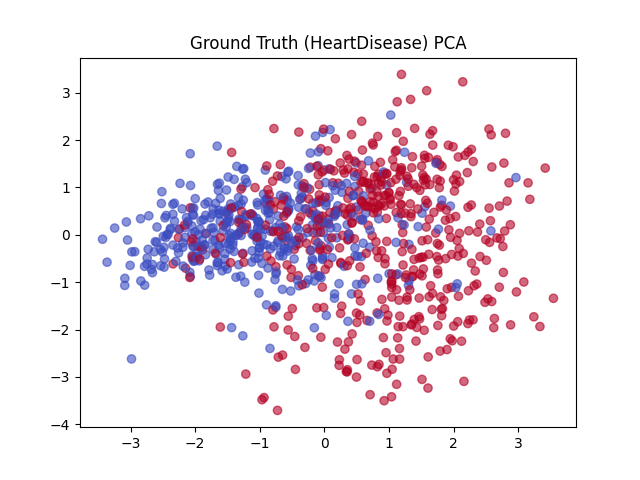
\includegraphics[width=0.6\textwidth]{images/ground_truth_pca.png}
    \caption{Visualização PCA do dataset com as classes reais (\textit{Ground Truth}) da Doença Cardíaca para fins de comparação com a Figura \ref{fig:kmeans}.}
    \label{fig:ground_truth}
\end{figure}

\end{document}
